\chapter[Interférence vs. exploitation et dynamique des populations
structurées][Interférence et populations structurées]{Interférence vs.
exploitation et dynamique des populations structurées}
\label{chap:amnat}

\vspace{2cm}
\begin{Spacing}{1}
\texttt{
Le Bourlot, Vincent, Thomas Tully and David Claessen, "Interference versus
Exploitative Competition in the regulation of Size-Structured Populations"\\
under review at The American Naturalist
}
\end{Spacing}
\vspace{2cm}


\lettrine[lines=3]{D}{ans le chapitre} précédent, nous avons pu voir le rôle
prépondérant que jouent les individus de grande taille dans la régulation des
populations de collembole \textit{Folsomia candida} élevées en laboratoire. Les
individus de grande taille impactent fortement la population par l'intermédiaire
des interactions entre individus et de la compétition pour les ressources. La
compétition est un des facteurs principaux dans la régulation de la dynamique
des populations et des communautés. Son effet peut être soit direct entre
plusieurs individus via la compétition par interférence, ou par l'intermédiaire
de la ressource dans la compétition par exploitation.

L'impact de la compétition par exploitation sur la dynamique des populations a
déjà été largement étudié, tant d'un point de vue empirique que théorique, mais
les effets de la compétition par interférence restent quant à eux mal compris.
Nous avons déjà donné des arguments empiriques quant au le rôle de
l'interférence dans la régulation de la dynamique des populations structurées
(Chapitre \ref{chap:sp}), mais à ce jour, il n'existe pas encore de cadre
théorique aux effets de la compétition par interférence sur les populations structurées.

Nous étudions dans ce chapitre les effets de différents niveaux de compétition
intra-spécifique par interférence sur la dynamique d'une population structurée
en taille. Nous basons notre étude sur un modèle ressource -- consommateur
physiologiquement structuré \autocites[modèle de ][]{kooijman1984a} prenant
en compte des interactions directes entre les individus, autorisant ainsi un
gradient depuis une compétition purement par exploitation à une compétition
totalement dominée par l'interférence. Nous paramétrons notre modèle en
utilisant les données issues des suivis expérimentaux de populations de
collemboles \textit{Folsomia candida}.

Notre modèle prédit une variété de dynamiques possibles suivant le niveau de
compétition par interférence imposé. A un faible niveau d'interférence, notre
modèle se comporte de manière similaire au modèle classique de Kooijman et Metz.
Un niveau légèrement supérieur d'interférence agit comme une force
stabilisatrice sur les cycles de générations causés par les juvéniles. A niveau intermédiaire, des
géants émergent dans la populations et commencent à la dominer. Enfin, à un
niveau très élevé d'interférence, un nouveau type de cycles apparaît que l'on
appelle ``cycles causés par l'interférence''. Nos résultats théoriques
permettent d'apporter un nouvel éclairage dans l'interprétation des dynamiques de la
structure en taille des populations de collemboles élevées au laboratoire. Les
travaux présentés dans ce chapitre feront l'objet d'une publication présentée
dans l'Annexe \ref{An:AmNat}.

\section{Éléments de méthodologie}


\subsection{Définition du modèle}

\subsubsection{Paramètres du modèle}

Notre modèle repose sur celui développé par
\textcites[KM-model][]{kooijman1984a} et \textcites{de-roos1992a}. Ce modèle
est un modèle mécaniste qui défini les processus au niveau individuel et laisse
la dynamique émerger au niveau de la population. Les paramètres du
modèle sont tirés des suivis expérimentaux des populations de collembole
présentés dans le Chapitre précédent. 


\subsubsection{Densité dépendance}

L'objectif de ce modèle est de prendre en compte les
processus d'interférence dans les mécanismes de densité dépendance qui régulent la population. Nous avons
défini l'état physiologique d'un individu par sa longueur corporelle $l$. Cette
longueur varie de la taille à la naissance $l_b$ à la taille maximum atteignable
sans aucune compétition $l_m$. Nous décrivons les interations individuelles au
travers de la fonction $A(t,l)$. Cette fonction que l'on appelle fonction
``d'accès à la ressource'' dépend de la densité de la population telle qu'elle
est resentie par un individu, en fonction de sa taille. Cette densité resentie,
notée $\eta (t,l)$, repose sur le fait qu'un individu de petite taille est plus
impacté par la présence d'un individu de grande taille que l'inverse. Les
paramètres de la fonction $A$ nous permettent alors d'ajuster le niveau de
compétition par interférence dans la population. Cette fonction est définie
comme suit, avec $\eta _H$ un coefficient de demi-saturation:

\begin{equation}
\label{eq_an1}
A(t,l)=1-\frac{\eta(t,l)}{\eta_H+\eta(t,l) }  
\end{equation}

La densité ressentie $\eta$ est définie pour un individu de taille $l$, au temps
$t$, par:

\begin{equation}
\label{eq_an2}
\eta(t,l)=\int_{l_b}^{l_m} \! C(l,\lambda)\cdot n(t,\lambda)\cdot\lambda^2\, \mathrm{d}\lambda
\end{equation}

La densité de la population ressentie par un individu dépend donc de la
structure effective de la population, et d'une fonction de compétition $C(\lambda ,l)$.
Cette fonction de compétition représente la supériorité d'un individu de taille
$\lambda$ sur un individu de taille $l$ en fonction de la différence de taille
entre les deux:

\begin{equation}
\label{eq_an3}
C(l,\lambda) = \mathrm{max}\left[ 0.01,\, 1+I\cdot(\lambda-l) \right]
\end{equation}

où $I$ est le paramètre d'interférence qui permet de régler le niveau de
compétition par interférence dans la population. $I=0$ conduira à une population
régulée uniquement par de la compétition par exploitation. A l'inverse, une
valeur de $I$ très élevée indique une forte domination de l'interférence sur
l'exploitation.

\subsubsection{règle du $\kappa$ et taux individuels}

\begin{figure}[!ht]
\begin{center}
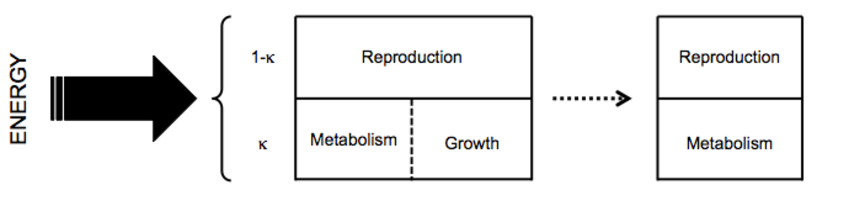
\includegraphics[width=0.95\textwidth]{1_CorpsDeThese/Resumes/Fig/AN01}
\caption[\lofimage{1_CorpsDeThese/Resumes/Fig/AN01}Règle du
$\kappa$]{Schéma de la règle du $\kappa$ et de ses implication}
\label{fig:AN1}
\end{center}
\end{figure}

Outre les interactions entre individus, le modèle se base sur les règles
d'allocation dynamique du budget énergétique \autocites{kooijman2000a}. Une fois la règle fixée, on peut en
dériver les taux vitaux individuels. 

Nous nous basons sur la règle d'allocation appelée règle du
$\kappa$ ($\kappa$-rule), schématisée par la Figure \ref{fig:AN1}. Cette règle
suppose qu'une proportion $\kappa$ de l'énergie acquise par un individu est
allouée à la maintenance (métabolisme) et à la croissance, le reste ($1-\kappa$)
étant attribué à la reproduction. Cela implique automatiquement qu'un individu à sa
taille maximum continue de se reproduire, ce qui n'est pas toujours le cas pour
d'autres règles d'allocation de l'énergie (voir Annexe \ref{An:AmNat},
Supplementary Materials \ref{subsec:SupMat4}). Lorsque l'individu ne grandit
plus, l'énergie est alors divisé en une fraction fixe pour couvrir le
métabolisme et le reste pour la reproduction. Si l'énergie acquise diminue, le
métabolisme étant fixé par la taille de l'individu, la quantité
allouée à la reproduction diminue. Si l'énergie acquise n'est pas suffisante
pour couvrir l'intégralité du métabolisme, l'individu meure.

On suppose que l'acquisition de la ressource est proportionnelle à $l^2$
et que le métabolisme est proportionnel à $l^3$, cette règle d'allocation de
l'énergie nous permet alors de définir les taux vitaux individuels tels que
décrit dans la Table \ref{tab:ANEq}. Le détail de la dérivation des équations du modèle
est disponible dans les Supplementary Materials \ref{subsubsec:SupMat21} de
l'Annexe \ref{An:AmNat}. 

\begin{table}
\centering
\caption{\label{tab:ANEq} Equations du modèle d'après la règle du $\kappa$.}
\begin{tabular}{cl}
\hline 
\hline
&\\
Equation & Description \\
\hline
	$\displaystyle{A(t,l)=1-\frac{\eta(t,l)}{\eta_{H}+\eta(t,l)}}$ & Access to the
	resource\\
	&\\
	$\displaystyle{\eta (t,l) = \int\limits_{l_b}^{l_m} C(l,\lambda)\cdot
	n(t,\lambda)\cdot \lambda^2\,\text{d}\lambda}$ & Experienced population
	density\\
	&\\
	$\displaystyle{C(l,\lambda) = \text{max}[0.01,\, 1+I\cdot(\lambda-l)]}$ &
	Competition function \\
	&\\
	$\displaystyle{g(t,l) = \gamma\cdot(l_m \cdot A(t,l)-l)}$ & Growth rate\\
	&\\
	$\displaystyle{b(t,l) = r_m \cdot A(t,l)\cdot l^2}$ & Birth rate if $l\geq
	l_j$\\
	&\\
	&\\
	$\displaystyle{\frac{\partial n(t,l)}{\partial t}+ \frac{\partial
	g(t,l)\cdot n(t,l)}{\partial l} = -\mu \cdot n(t,l) }$ & Population level
	equation\\
	&\\
	$\displaystyle{g(t,l_b)\cdot n(t,l_b) = \int\limits_{l_b}^{l_m} b(t,l)\cdot
	n(t,l) \, \text{d}l}$ & Boundary conditions \\
\hline 
\end{tabular} 
\end{table}

\subsubsection{Minimum vital d'accès aux ressources}
Nous définissons le minimum vital d'accès aux ressources comme la quantité $A^*$
telle que la croissance individuelle est nulle.

\begin{equation}
\label{eq_an4}
A^*(l) = \frac{l}{l_m}
\end{equation}
Bien que dépendante de $l$,
cette quantité est analogue au $R^*$ de Tilman dans le sens où elle définit des
conditions minimums permettant la croissance des individus. 

Les paramètres utilisés dans ce modèle sont rappelés dans la Table
\ref{tab:ANparam}. Les données expérimentales permettant de justifier ces
données sont présentées dans les Supplementary Materials \ref{subsec:SupMat1} de
l'Annexe \ref{An:AmNat}. 

\begin{table}
\caption{\label{tab:ANparam}Variables et paramètres pour \textit{Folsomia
candida}}
\begin{tabular}{cccl}
\hline
\hline 
 & & &\\
 Objects and  & Default values & Units & Description\\ 
symbols & & &\\
\hline
	$i$-state variable & & & \\ 
	$l$ &   & mm & Individual length \\ 
	Parameters & & & \\ 
	$l_{b}$ & 0.25 & mm & Length at birth \\ 
	$l_{j}$ & 0.6 & mm & Length at maturity \\ 
	$l_{m}$ & 3.0 & mm & Length at infinite\\
	& & &  resources \\ 
	$\gamma$ & 0.015 & d$^{-1}$ & Van Bertalanffy growth rate \\ 
	$\eta_{H}$ & 1000 & individuals & Half saturation constant \\ 
	$\mu$ & 0.0065 & d$^{-1}$ & Background mortality \\ 
	$r_{m}$ & 3.0 & d$^{-1}$mm$^{-2}$ & Reproduction rate \\ 
	$\kappa$ & 0.7 & -- & Fraction of energy \\
	  &   &   & intake allocated \\
	  &   &   & to reproduction \\ 
	  $I$ & 0 & -- & Level of interference\\
\hline 
\end{tabular} 
\end{table}

\subsubsection{Intégration au niveau population}

Au niveau de la population, le nombre d'individus au temps $t$ est donné par
\begin{equation}
\label{eq_an5}
\int_{l_b}^{l_m}\!n(t,l)\,\mathrm{d}l
\end{equation}
où $n(t,l)$ est le nombre d'individus de taille $l$ au temps $t$. La dynamique
de la population est alors donnée par les équations et conditions initiales
suivantes \autocites{kooijman1984a,de-roos1997a}:
\begin{align}
\label{eq_an6}
\frac{\partial n(t,l)}{\partial t}+\frac{\partial g(t,l) \cdot n(t,l)}{\partial l}=-\mu \cdot n(t,l) \\
g(t,l_b) \cdot n(t,l_b)= \int_{l_b} ^{l_m} \! b(t,l)\cdot n(t,l)\, \mathrm(d)l
\\ n(0,l)=\Psi(l)
\end{align}

\subsection{Analyse de bifurcation}

Afin d'étudier le rôle de l'interférence dans les dynamiques produites par notre
modèle, nous avons réalisé une analyse de bifurcation sur le paramètre $I$ du
modèle. Bien que cette analyse ne soit pas une analyse de continuation à
proprement parler, elle nous permet d'identifier les intervalles de paramètre
correspondant à différents types de dynamiques. 

Le principe de cette analyse est comme suit: (i) une première simulation est
exécutée avec la valeur initiale du paramètre dit de bifurcation (ici $I$)
jusqu'à ce que la population ait quitté le régime transitoire; (ii) l'état final
de la population (soit sa distribution à la fin de la simulation) est utilisé
comme état initial d'une nouvelle simulation; (iii) le paramètre d'interférence
est incrémenté; et (iv) le processus est répété jusqu'à exploration de
l'ensemble de l'intervalle voulu. Notons que cette analyse peut également être
réalisée avec des valeurs décroissantes du paramètre de bifurcation, ce qui peut
permettre d'identifier des zones de bistabilité. 

Dans un premier temps, cette analyse a été réalisée pour une valeur fixe des
paramètres excepté le paramètre de bifurcation $I$. Puis, sachant que la
mortalité a un fort effet sur la dynamique de ce type de modèle, cette analyse
a été faite pour des valeurs successives de mortalité avec le paramètre $I$
comme paramètre de bifurcation, et pour des valeurs successives d'interférence
avec le paramètre de mortalité $\mu$ comme paramètre de bifurcation. Ainsi,
l'ensemble de l'espace $(I,\mu)$ a été quadrillé pour des valeurs de $I$ de 0 à
3 et des valeurs de $\mu$ de 0.001 à 0.02

\section{Résultats}

Nous nous intéressons dans un premier temps à l'effet du niveau de compétition
par interférence pour une valeur assez faible de mortalité ($\mu = 0.0065$,
Figure \ref{fig:AN2}). 

\begin{figure}[!ht]
\begin{center}
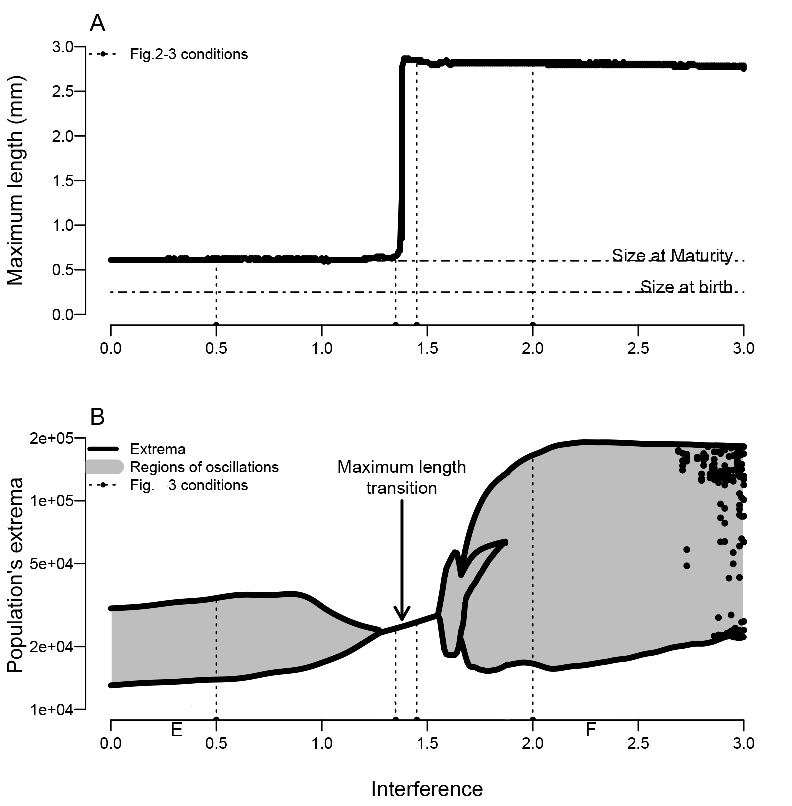
\includegraphics[width=0.95\textwidth]{1_CorpsDeThese/Resumes/Fig/AN02}
\caption[\lofimage{1_CorpsDeThese/Resumes/Fig/AN02}Bifurcation sur le
niveau d'interférence]{Taille maximum atteinte dans la population (A) et extrema
de la population (B, nombre d'individus) en fonction du niveau de compétition par interférence $I$ pour une
valeur constante de mortalité ($\mu = 0.0065$). Les lignes pointillées
représentent les valeur d'interférence des simulations présentées en Figure
\ref{fig:AN3}. Les zones grisées marquent les zones ou la population est
cyclique. La flèche marque la transition de taille maximum atteinte.}
\label{fig:AN2}
\end{center}
\end{figure}

On constate dans un premier temps qu'un niveau suffisamment élevé de compétition
par interférence ($I=1.4$) provoque une transition dans la taille maximum
atteinte par les individus (Figure \ref{fig:AN2}A). Lorsque le niveau
d'interférence est plus faible que cette valeur, la taille maximum atteint ($l=0.63mm$) reste proche de la taille à
maturité ($l_j=0.6mm$). Au delà de la valeur critique, la taille atteinte
($l=2.85mm$) se rapproche fortement de la taille maximum atteignable
($l_m=3mm$). 

De plus, la Figure \ref{fig:AN2}B montre trois régions distinctes: (i) à faible
interférence, la population est cyclique; (ii) pour un niveau intermédiaire de
compétition par interférence, la population est stable; et (iii) pour une forte
interférence, la population cycle autour d'un nouveau type de cycles de plus
grande amplitude que les précédents. 

\subsection{Des cycles dirigés par les juvéniles}

Les modèles PSP classiques prédisent qu'à faible mortalité, la différence de
capacité de compétition entre les juvéniles et les adultes conduit à des cycles
de génération dirigés par les juvéniles \autocites{de-roos1992a,de-roos1997a}.
La Figure \ref{fig:AN3}abc montre la dynamique de la population pour un faible
niveau d'interférence ($I=0.5$). On observe sur le diagramme structure-temps (a)
que la dynamique cyclique correspond à des vagues successives de recrutement de
juvéniles avec des adultes ne dépassant que très peu la taille à maturité. Cette
dynamique est caractéristique des cycles de génération dirigés par les juvéniles
\autocites{de-roos1992a,de-roos2003a}.

\afterpage{%
    \clearpage% flush all other floats
    \ifodd\value{page}
    %\else% uncomment this else to get odd/even instead of even/odd
        \expandafter\afterpage% put it on the next page if this one is odd
    \fi
    {%
    \begin{figure}[p]
        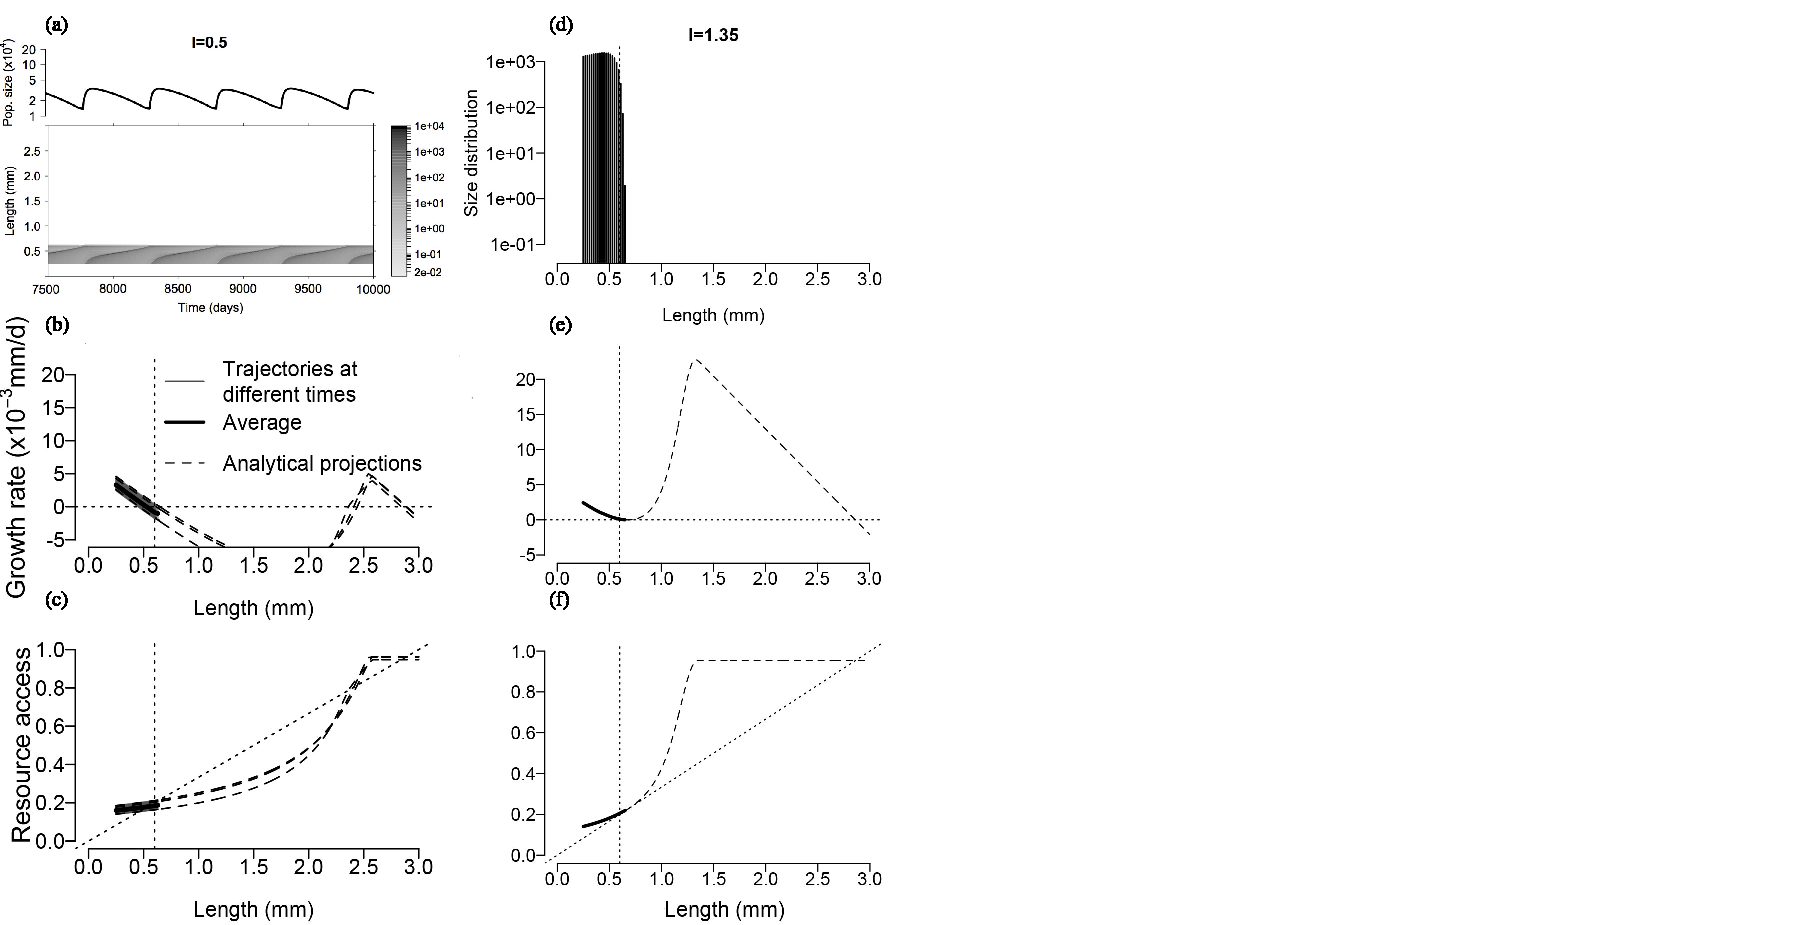
\includegraphics[width=\textwidth]{1_CorpsDeThese/Resumes/Fig/AN03}
        \caption{Exemples de dynamiques pour quatre valeurs d'interférence: 0.5,
1.5, 1.45 et 2.0. La première ligne de panels (a,d,g,j) montre soit la
dynamique de la structure à l'aide d'un diagramme structure-temps (a,j), soit la
distribution de la taille si elle est stable dans le temps (d,g). La seconde
ligne (b,e,h,k) représente le taux de croissance en fonction de la longueur
corporelle\ldots}\label{fig:AN3}
    \end{figure}
    \clearpage
    \begin{figure}[p]
		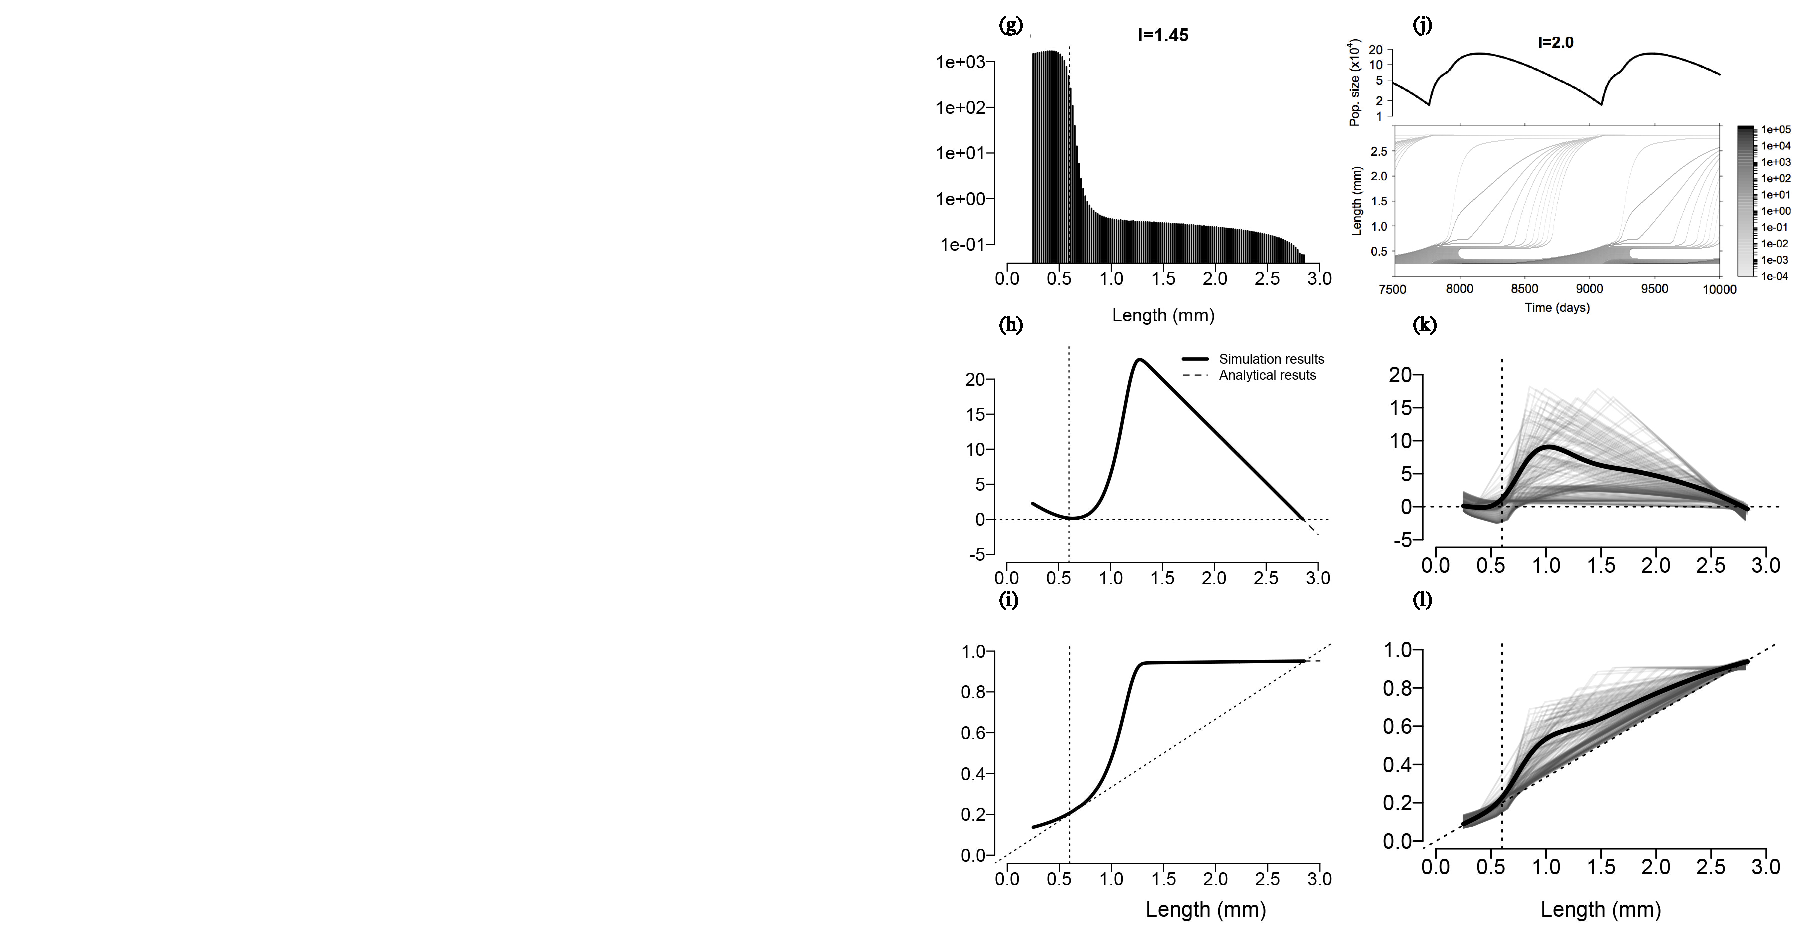
\includegraphics[width=\textwidth]{1_CorpsDeThese/Resumes/Fig/AN04}
        \caption*{\ldots Lorsque la dynamique est cyclique, plusieurs
        trajectoires sont présentées, ainsi que leur moyenne en trait épais.La ligne pointillée
horizontale est le 0, la ligne verticale marque la taille à maturité. Enfin, la
dernière ligne de panels (c,f,i,l) présente l'accès à la ressource. La ligne
verticale marque la taille à maturité, la ligne oblique marque l'accès minimum
requis $A^*$. Pour le taux de croissance et l'accès aux ressources, les lignes
tiretées représentent les projections analytique des fonctions tracées.}
    \end{figure}
    \clearpage
    }%
}

Les Figures \ref{fig:AN3}b et c montrent le taux de croissance et l'accès aux
ressources pour cette dynamique. Le taux de croissance décroît
quasi-linéairement avec la taille, de façon très similaire au modèle classique
sans interférence. L'accès aux ressources est très légèrement croissant mais
devient rapidement inférieur à $A^*$ pour tous les individus après la maturité. 

\subsection{Un équilibre stable avec des petits ou des géants}

Pour des valeurs intermédiaires de compétition par interférence, l'avantage
que les grands individus retirent de l'interférence contrebalance la compétition
par exploitation imposée par les juvéniles. Ceci vient contrer les mécanismes
de déséquilibre compétitif à l'origine des cycles de génération, et tend à
stabiliser la population (Figure \ref{fig:AN3}d-i).

Pour une valeur d'interférence sous le seuil critique de $I=1.4$, la dynamique
se stabilise autour d'une distribution étroite de la taille corporelle (Figure
\ref{fig:AN3}d). Le taux de croissance et l'accès à la ressource ont tendance à
se courber vers le haut pour les plus grands individus, mais la courbure n'est
pas suffisante pour permettre à l'accès au ressources de rester au dessus de
$A^*$, et les individus s'arrêtent de grandir rapidement après la maturation (Figure
\ref{fig:AN3}ef).

Au delà de ce seuil critique, la courbure est suffisante pour que l'accès aux
ressources soit toujours supérieur à $A^*$ et le taux de croissance soit
toujours positif (Figure \ref{fig:AN3}hi). Après un ralentissement de leur
croissance proche de la maturité (``goulet d'étranglement de la croissance''), les individus peuvent
reprendre une croissance rapide jusqu'à des tailles très élevées. La
distribution de la taille dans la population est alors très asymétrique vers les
juvéniles, mais reste continue jusqu'à des tailles proches de la taille maximum
possible $l_m$ (Figure \ref{fig:AN3}g). Les formes particulières des fonctions
de croissance et d'accès à la ressource s'expliquent d'abord par la faible
densité d'adultes au delà de $0.6mm$ et leur grande compétitivité, ils
sont donc rapidement capables de monopoliser la ressource et grandissent très
rapidement. La partie linéaire après $l=1.4mm$ est quand a elle la conséquence
de la forme naturelle de la fonction de croissance de Von Bertalanffy. 

\subsection{Des cycles induits par l'interférence}

La bifurcation sur l'interférence montre l'apparition de cycles lorsque le
niveau de compétition par interférence est suffisamment élevé ($I>1.56$ Figure
\ref{fig:AN2}). La Figure \ref{fig:AN3} (j-l) montre le détail de la dynamique
pour une valeur de compétition par interférence de $I=2.0$. On constate sur le
diagramme structure temps (j) que les cycles dans la structure de la population
sont très différents des cycles de génération induits par les juvéniles (a). La
période des cycles a été multipliée par $3$ et l'amplitude est environ $7.5$
fois supérieure. Un cycle dans la dynamique commence par un pulse de naissance
qui fait fortement augmenter la taille de la population lorsqu'une cohorte
d'individus atteint la maturité. La population est alors multi-modale avec une majorité
de juvéniles, des adultes nouvellement matures et quelques vieux individus de
très grande taille. Après le pulse de naissance, les individus qui viennent de
maturer grandissent, ce qui réduit la ressource disponible pour les individus
les plus petits qui stoppent leur croissance. Deux groupes se forment, des
juvéniles de moins de $0.35mm$ et des juvéniles et jeunes adultes entre $0.5$ et
$0.75mm$. Pendant cette période, les adultes continent de se reproduire,
augmentant la densité de juvéniles. Les individus les plus vieux commencent
ensuite à mourir, diminuant progressivement la pression de compétition sur les
jeunes adultes qui atteignent à leur tour des tailles extrêmes. La pression de
compétition est cependant maintenue sur les plus petits juvéniles qui ne peuvent
pas grandir. Le nombre d'individus reproducteur commence alors à diminuer,
réduisant progressivement la taille de la population et la pression de
compétition due à l'interférence. Quand suffisamment d'adultes sont mort, la
pression de compétition a assez diminué pour que les plus petits juvéniles
reprennent leur croissance et maturent, provoquant un nouveau cycle dans la
dynamique. 

On constate sur le panel (k) que la position du goulet d'étranglement du taux de
croissance sur l'axe des X varie entre $0.33$ et $0.55mm$ suivant le moment dans
le cycle, mais reste systématiquement inférieur à la taille à maturité
$l_j=0.6mm$, ce qui provoque l'accumulation d'individus immature dans la
population. L'accès aux ressources (l) montre le même phénomène. Les individus
n'accèdent plus suffisamment aux ressources pour poursuivre leur croissance dont
le taux devient négatif (causant une mortalité accrue). Ils arrêtent donc leur
croissance à un stade immature, ce qui fait diminuer le nombre de reproducteur
et relâche progressivement la pression de compétition par interférence. C'est
précisément la position du goulet d'étranglement sous la taille à maturité qui
déstabilise la dynamique vers ces nouveaux cycles. 

\subsection{Bifurcation dans le plan $(I,\mu)$}

Le taux de mortalité basal $\mu$ étant connu pour affecter la dynamique des
populations structurées par taille, en stabilisant la dynamique vers un point
fixe lorsqu'il augmente, nous nous somme intéressé à son effet couplé à celui du
niveau de compétition par interférence. La Figure \ref{fig:AN4} montre le type
de dynamique obtenu en fonction de la position dans le plan de paramètres
$(I,\mu)$.

\begin{figure}[!ht]
\begin{center}
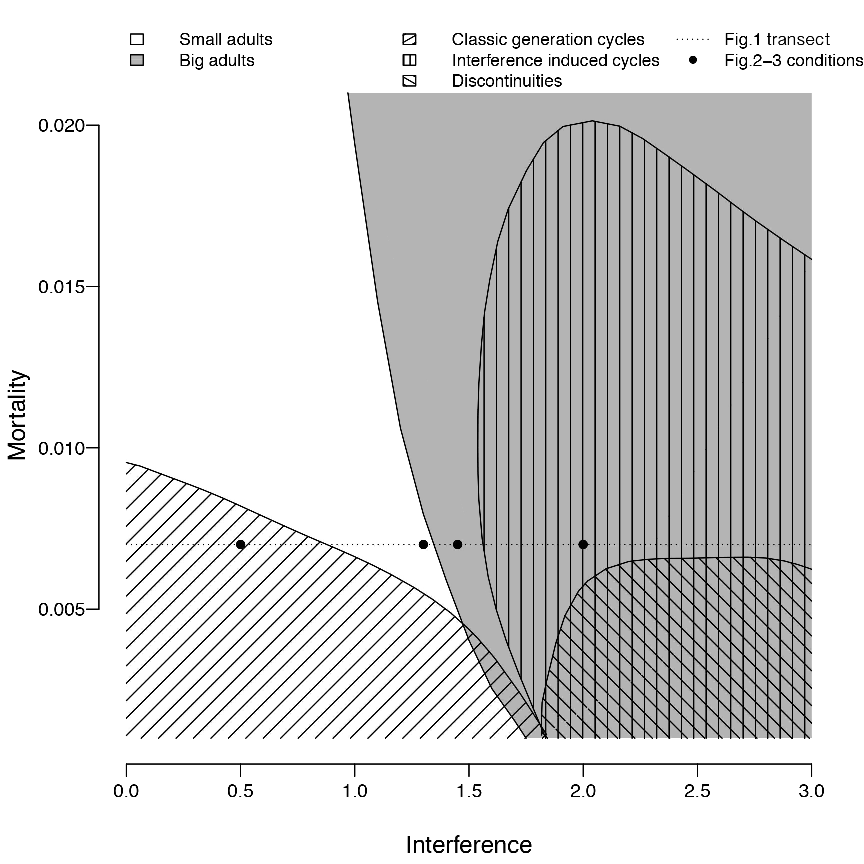
\includegraphics[width=0.95\textwidth]{1_CorpsDeThese/Resumes/Fig/AN05}
\caption[\lofimage{1_CorpsDeThese/Resumes/Fig/AN05}Diagramme de
bifurcation dans le plan $(I,\mu)$]{Diagramme de
bifurcation dans le plan $(I,\mu)$. Les régions sans hachure sont les régions
correspondant à un point fixe. Les hachures représentent le type de cycle
obtenu. La zone grise correspond à la zone de survie des individus de très
grande taille. La ligne pointillée et les points marquent respectivement la
bifurcation de la Figure \ref{fig:AN2} et les simulations de la Figure
\ref{fig:AN3}}
\label{fig:AN4}
\end{center}
\end{figure}

Dans un premier temps, on peut distinguer deux régions différentes sur ce
diagramme (régions blanches et grises) qui délimitent les zones où
la taille maximale atteinte est soit proche de la taille à maturité (en blanc),
soit proche de la taille maximum possible (en gris). Il est intéressant de noter
que la limite entre ces deux régions dépend assez peu de la mortalité basale
( $I$ entre $1.2$ et $1.6$).

On remarque également qu'en l'absence d'interférence, les cycles de génération
induits par les juvéniles sont stabilisés lorsque la mortalité basale augmente,
conformément à la théorie déjà établie \autocites{de-roos1997a}. Lorsque la
compétition par interférence est présente, cette stabilisation se produit pour
des valeurs plus basses de mortalité. De plus, l'augmentation du taux de
mortalité semble également stabiliser les cycles due à l'interférence, mais pour
des valeur très élevées ($\mu > 0.02$). 

A faible mortalité mais haut niveau d'interférence, la dynamique est irrégulière
et les résultats sont peu fiables à cause de problèmes numériques liés à
l'intégration des équations du modèle. En revanche, pour une interférence
intermédiaire et une faible mortalité, on peut observer une situation
intéressante. En effet, on constate qu'il existe une petite région où des cycles
de génération semblables à ceux dues aux juvéniles se maintiennent alors que la
taille maximum atteinte est proche de la taille maximum possible. Mais ces
cycles sont dégénérés et quelques individus parviennent de temps en temps à
s'échapper du goulet de croissance et atteindre des tailles géantes. Ces
individus sont rares et les dynamiques irrégulières. 

\section{Discussion}

Nous avons mis en évidence au cours de cette étude que la compétition par
interférence est une interaction qui, en conférant un avantage aux individus les
plus grands, vient contrecarrer les effets de la compétition taille dépendante
par exploitation. La dépendance à la taille de l'ingestion d'énergie et de son
utilisation confère un avantage aux individus les plus petits par la compétition
par exploitation \autocites{peters1986a,persson1998a,de-roos2013a} comme le
prédit la théorie du budget énergétique dynamique \autocites{kooijman2000a}.
Dans l'intervalle de niveaux de compétition par interférence que nous étudions
ici, l'équilibre compétitif entre les plus petits et les plus grands individus
bascule progressivement d'un avantage aux juvéniles, du à la compétition par
exploitation, à un avantage aux grands adultes, du à la compétition par
interférence. Entre les deux extrêmes, les compétitions par exploitation et
interférence s'équilibre et la population se stabilise. Les transitions observée
dans la Figure \ref{fig:AN2} sont très comparables à celles causées par des
modifications de la dépendance en taille de la compétition par exploitation,
telles que l'augmentation des pentes des fonctions allométriques pour le taux
d'attaque \autocites{persson1998a} ou pour le taux de consommation
\autocites{de-roos2003a}. Cependant, les mécanismes sous jacents restent très
différents. En effet, la transition vers des cycles dominés par les adultes dans
les études de \textcites{persson1998a} et \textcites{de-roos2003a} se produisent
pour des valeurs de paramètre peu réalistes. Déjà prédite par
\textcites{de-roos2003a}, notre étude propose une hypothèse alternative
conduisant à des cycles de génération dominés par les adultes.

Bien que les cycles induits par l'interférence ne soient pas strictement des
cycles dominés par les adultes (``adult driven generation cycles'') selon la
définition de \textcites{de-roos2003a}, ils partagent avec eux une
caractéristique essentielle, à savoir le fait que les oscillation reposent sur
la domination compétitive des individus les plus grands qui empêchent une
nouvelle génération de dominer la population tant qu'ils sont suffisamment
nombreux. Dans ce sens, les cycles induits par l'interférence font partie
des cycles dominés par les adultes.  

\subsection{Détecter la compétition par interférence dans des populations
naturelles} 

Le cannibalisme est un autre mécanisme qui confère un avantage aux
plus grands individus d'une population sur les plus petits en les protégeant de la
compétition par exploitation \autocites{claessen2000a,claessen2002a}, et peut
ainsi conduire à la stabilisation des cycles dominés par les juvéniles et
l'émergence d'individus de grande taille. Ces similarités font qu'il est
nécessaire d'avoir des clés permettant de discriminer différentes causes pouvant
mener aux même observations dans des populations naturelles. 

D'après nos résultats théoriques, plusieurs critères peuvent être utilisés pour
identifier le rôle de la compétition par interférence dans la dynamique d'une
population structurée. 
\begin{enumerate*}[label=(\roman*)]
\item L'observation la plus évident de l'effet de l'interférence est l'émergence
de géants dans la population. Bien que d'autres cause puissent provoquer cette
émergence telles que le cannibalisme ou une niche spécifique pour les plus
grands individus, combiné aux éléments suivant, c'est un indice en faveur
de la compétition par interférence. 
\item La présence d'un goulet d'étranglement de la croissance est un signe fort
de l'action d'une compétition par interférence assez intense.
\item Ce goulet d'étranglement provoque une distribution de la taille
fortement asymétrique en faveur des plus petits individus dans une population
stable. 
\item Dans une population cyclique, cela résulte en une distribution
multi-modale.
\item Dans les deux cas, les trajectoires de croissance individuelles
ressemblent à une double courbe de croissance. Les individus subissent un
ralentissement violent de la croissance autour de la maturité avant une
accélération brutale passé le goulet d'étranglement. 
\item L'observation des traits d'histoire de vie individuels permets donc de
distinguer les cycles causés par l'interférence des cycles dominés par les
juvéniles. Dans le dernier cas, les individus grandissent rapidement et
s'arrêtent après maturation alors que dans le premier cas la croissance s'arrête
vers la maturation pour ne reprendre que si la cohorte adulte dominante a
suffisamment diminuée. 
\item Enfin, dans le cas où les données individuelles ne sont pas accessibles,
le ratio du temps de maturation moyen par la période des cycles tel que défini
par \textcites{murdoch2002a} permet également de faire la distinction entre les
différents cycles. Comme expliqué en introduction de cette thèse
(Section \ref{modelPopStru} page \pageref{modelPopStru}), une valeur du ratio
autour de $1$ correspond à des cycles de génération. Dans notre modèle, les
cycles dominés par les juvéniles ont un ratio autour de $0.8$ alors que les cycles induits par l'interférence ont un
ratio proche de $1.5$. Ainsi, des cycles de génération avec un ratio supérieur
à 1 pourraient être une indication du rôle de l'interférence. Cela pourrait par
exemple être le cas pour les saumons dans la baie de Bristol (ratio$=1.2$) ou de
la rivière Togiak ($1.3$), la morue d'Iceland ($1.6$), le castor de Californie
(1.6), ou l'ours noir du Yukon \autocites[1.5,][]{murdoch2002a}. Ces espèces
étant territoriales, elles sont en effet susceptibles à la compétition intra-spécifique par interférence. 
\end{enumerate*}

\subsection{L'interférence dans nos populations expérimentales}

Nous avons montré dans le Chapitre \ref{chap:sp} que nos populations
expérimentales de collemboles se caractérisent systématiquement par
l'existence de plusieurs modes dans la distribution de la taille des individus.
Généralement deux, un mode assez dense de juvéniles dont la taille est proche de
la taille à la naissance, et un mode d'adultes dont la taille est très
supérieure à la taille à maturité (parfois jusqu'à plus de trois fois
supérieur). Exceptionnellement, un troisième mode peut être observé, on a alors
un premier mode de juvéniles, un mode avec des petits adultes et un mode avec
des grands adultes. Mais nous avons montré que cette situation n'était stable
que localement, et ne pouvait être atteinte qu'avec des conditions initiale de
distribution de la taille très particulières qui ne se retrouvent quasiment
jamais hors de l'initialisation des populations.

De plus, nous avons montré que les individus de grande taille jouent un rôle
prépondérant dans la dynamique de la population notamment en empêchant la
croissance des juvéniles lorsque les cohortes d'adultes sont suffisamment
denses. 

Ces observations recoupent ainsi plusieurs des critères proposés à l'issue de
notre étude théorique pour identifier le rôle de la compétition par
interférence. Cette analyse apporte des arguments supplémentaires pour confirmer
le rôle de la compétition par interférence dans la dynamique des populations de
collemboles, et confirment ainsi du même fait l'intérêt des méthodes empiriques
employées dans l'étude précédente pour extraire le rôle de
l'interférence des données.

\section{En conclusion}

Notre objectif était ici d'étudier les conséquences de la compétition taille
dépendante par interférence sur la dynamique des populations, permettant ainsi
de compléter les résultats existants sur la compétition par exploitation et le
cannibalisme comme mécanismes intra-spécifiques de régulation des populations.
Nous avons donc développé un modèle simple de dynamique de populations physiologiquement
structurées qui à notre avis rassemble les aspects essentiels de la compétition
intra-spécifique par interférence. Ce modèle n'a ainsi pas pour vocation de
prédire précisément des dynamiques de populations, bien qu'il ait été paramétré
pour les Collemboles \textit{Folsomia candida}, mais plutôt de démontrer les
conséquences dynamiques de la compétition par interférence. La comparaison avec
nos données expérimentales issues des populations de collemboles montre qu'il
est possible de détecter le rôle de la compétition par interférence dans des
populations expérimentales ou naturelles. 

Dans notre cas, nous avons pu apporter de nouveaux éléments confirmant le rôle
de la compétition par interférence dans les dynamiques des populations de
collemboles, mais il reste encore des différences entre le modèle et les séries
temporelles observées, et les mécanismes détaillés à l'oeuvre dans les
populations expérimentales ne sont encore pas éclaircis. Dans le Chapitre
suivant, nous avons mené en parallèle deux études expérimentales afin de mieux
comprendre la façon dont les individus se répartissent l'accès à la ressource,
et le rôle des individus de différentes tailles dans la dynamique de la structure
des populations.
